\chapter{Community concept}
\label{CommunityConcept}
%I dette kapitel skal konceptet bag TonePrint communitiet forklares med udgangspunkt i at der tilsidst skal tages et valg af hvilken det vi skal hjælpe med at udvikle.\\
Based on the description of TC Electronics development process in \autoref{InterviewConclusion}, the current task is to develop conceptual models, which describes the functionalities and use cases of the TonePrint Community. The scope of this phase is to discover which tasks that lay ahead the development of the TonePrint Community, while focusing on user involvement and user experience. \\

\section{Conceptual model}
\label{ConceptualModel}
In \parencite[][17]{PDF:Henderson2012} a conceptual is descried  as "\textit{A high-level description of an application. It enumerates all concepts in the application that users can encounter, describes how those concepts relate to each other, and explains
how those concepts fit into tasks that users perform with the application.}"

\begin{figure}[H]
	\centering
	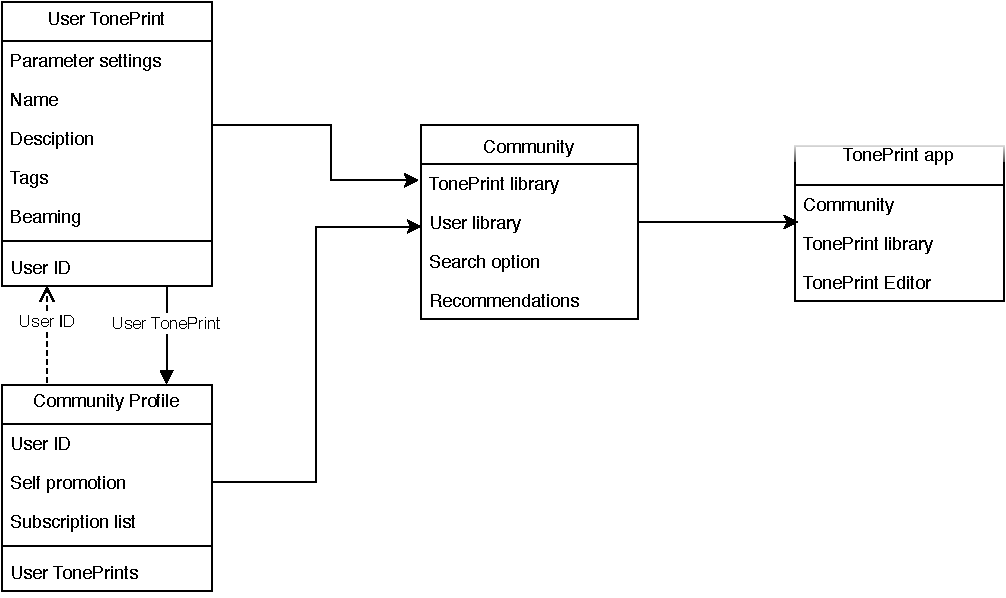
\includegraphics[width=0.85\textwidth]{CommunityFirstDraft.pdf}
	\caption{a graphical overview of the TonePrint Community concept}
	\label{fig:CommunityConceptualModel}
\end{figure}

\subsection{Use case}

\begin{figure}[H]
	\centering
	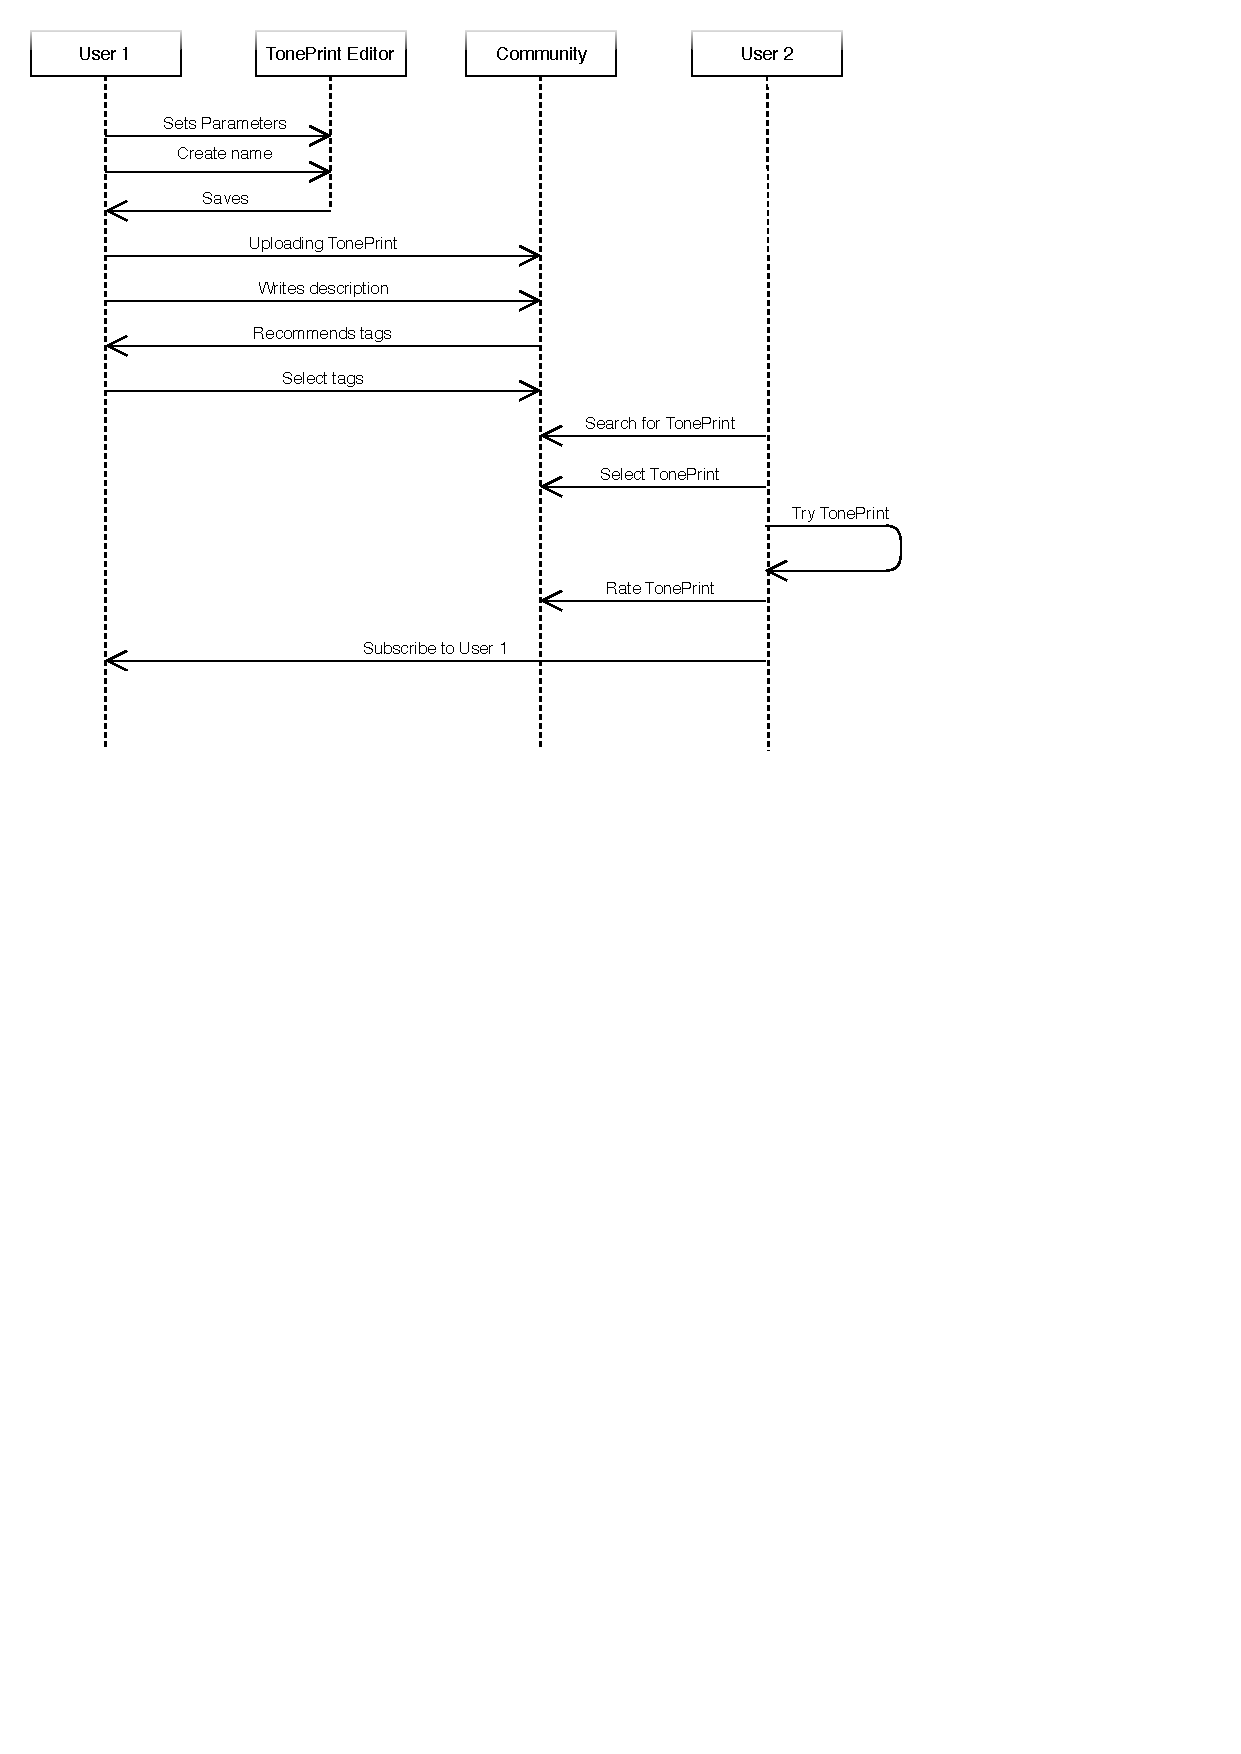
\includegraphics[width=0.85\textwidth]{CommunityUseCaseOne.pdf}
	\caption{a graphical overview of the TonePrint Community use case}
	\label{fig:CommunityConceptualUseCase}
\end{figure}